\chapter{Android Brukerveiledning}
Lag en demoapp som bruker azure mobile service og azure aad for autentisering. Om man har en app allerede følger man tutorialen som angitt, men kopierer heller den nye koden inn i din eksisterende app. 
\\
\\
Brukerveiledningen har tatt utgangspunkt i følgende brukerveiledninger fra Microsoft:
\\\url{http://azure.microsoft.com/en-us/documentation/articles/mobile-services-android-get-started/}
\\\url{http://azure.microsoft.com/en-us/documentation/articles/mobile-services-android-get-started-users/}
\\\url{http://azure.microsoft.com/en-us/documentation/articles/mobile-services-how-to-register-active-directory-authentication/}
\\
\\
Du skal ikke trenge å lese noen andre toturials enn denne med mindre du mangler en Azure Active Directory og Android Studio installasjon.


\section{Del 1 - Lag en mobile service i azure og eksempel-app}
\begin{enumerate}
\item Logg inn i management portalen og opprett en ny mobile service.
\\
\begin{figure}[H]
    \centering
    \setlength{\fboxsep}{0pt}%
    \setlength{\fboxrule}{1pt}%
    \fbox{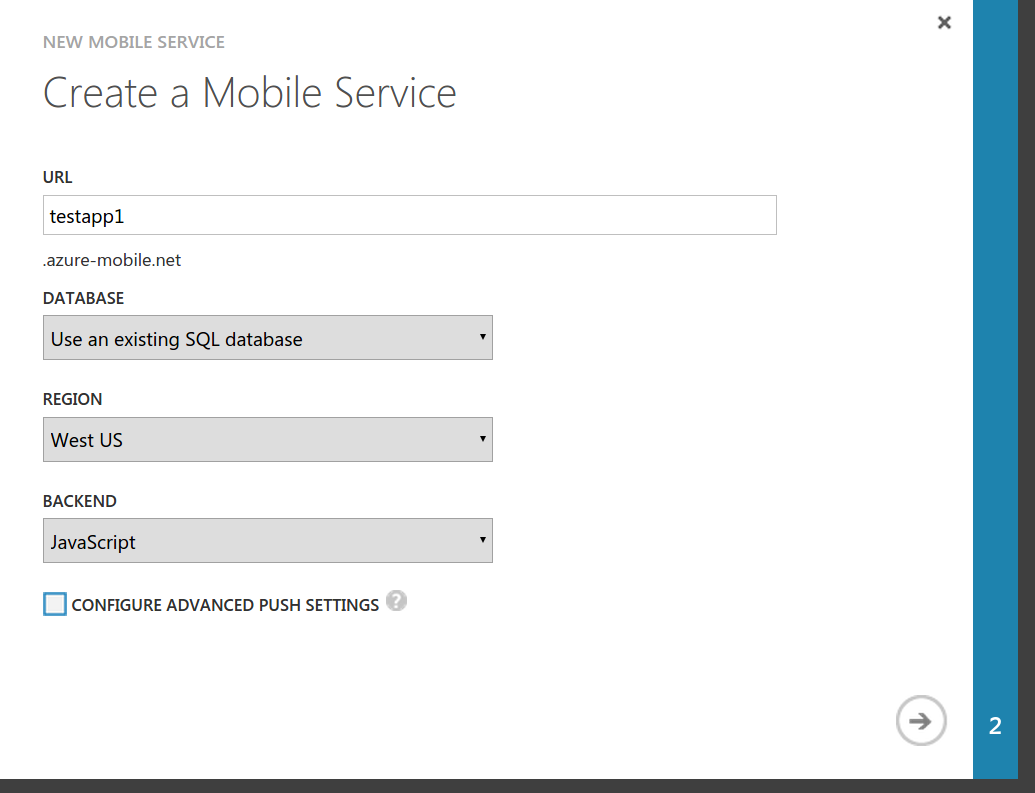
\includegraphics[scale=0.30]{graphics/veliedninger_implementeringAndroid/01-CreateMobileServices.png}}
    \caption{Creating a Mobile Service in Azure}
    %\label{fig:MobileServices}
\end{figure}

\\
\item Opprett navnet du vil at appen skal ha i AzureAD (URL), gjør gjerne dette så beskrivende som mulig.
\\
\item Velg type database du ønsker, her kan du bruke eksisterende SQL database, opprette ny SQL database eller opprette en gratis 20MB SQL database. Databasen må ligge i Azure eller være knyttet til Azure allerede om du skal bruke en eksisterende database.
\\
\begin{itemize}
\item “Region” sier hvor mobile servicen skal lagres, microsoft anbefaler å ha mobile service og database lagret i samme “region”.
\item “Backend” er for å legge inn backend API i tillegg til de spørringene en bruker allerede kan gjøre mot databasen.
\item Sett parametere for databasen. Skriv gjerne ned dette på et sikkert sted, kan hende det tar tid før man får bruk for denne informasjonen igjen. Gjentar at Microsoft anbefaler at databasen ligger i samme region som mobile-service, men dette er ikke et krav.
\end{itemize}
\bigskip

\item Etter at du har opprettet appen går du til Mobile Services i Azure portalen. Velg “Android”, deretter klikk på “create a new android app”
\\
\item Om du allerede har Android studio hoppe over dette punktet. Har du den ikke så last ned og installer android studio.
\\
\item Klikk på create table. Denne oppretter det du trenger for og kjøre eksempelappen. Last ned eksempelappen, det er denne appen denne tutorialen har tatt utgangspunkt i.
\\
\item Åpne appen i android studio, og la android studio kjøre bakgrunnsprosesser ferdig før du gjør noe. Du ser dette på nederste statuslinje i programmet. 
Om Android studio ikke vil godta sertifikatet som følger med prosjektet du har lastet ned så er dette kun knyttet til en https: kobling for og laste ned siste versjon av gradle. Denne pakken kan du hente over http kobling også, om du ønsker en rask løsning på dette.
\\
\begin{itemize}
\item Sertifikatfeilen lå i nedlastningen av siste gradle versjon. Rett opp dette ved å gå inn i filen gradle-wrapper.properties og endre distributionUrl fra https://... til http:// . Filen ligger i prosjektet under /gradle/wrapper/
\item Om Android studio kjører som det skal og ikke gir feilmeldinger kan du kjøre appen nå uten autentisering. Pakken du har lastet ned har automatisk lagt inn knytning til mobile service med uri og key. 
\item Om android sier du må laste ned noen sdk-er, følg bare anbefalte forslag fra android studio. 
\end{itemize}
\bigskip
\begin{figure}[H]
    \centering
    \setlength{\fboxsep}{0pt}%
    \setlength{\fboxrule}{1pt}%
    \fbox{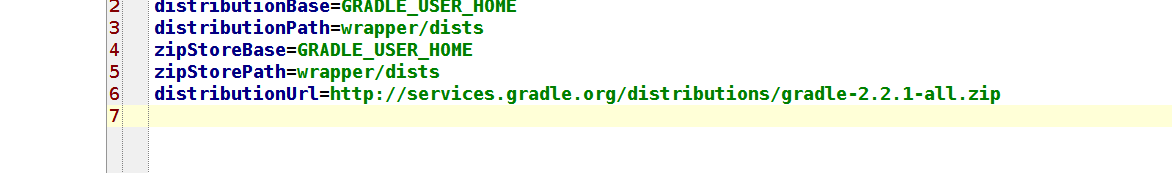
\includegraphics[scale=0.30]{graphics/veliedninger_implementeringAndroid/01-URLchange.png}}
    \caption{Skjermdump fra gradle-wrapper.properties}
    %\label{fig:MobileServices}
\end{figure}

\\
\item Appen skal nå virke, selv om den er svært enkel. 
\\
\item Sjekk gjerne at du finner igjen oppgavene du lagrer i todolisten i databasetabellen i Azure. Appen og databasen er ikke brukerstyrt, så om du installerer appen på flere telefoner, vi alle telefonene få opp det samme.
\end{enumerate}

\section{Del 2 - Legg inn autentisering i applikasjonen.}
For og kunne bruke azure ad som identity provider i appen må dette registrerers både i app koden, i Azure Mobile Service i Azure og i Azure Active Directory. Denne toturialen forutsetter at du har registrert en app i Azure Mobile Service, slik som i del 1 av denne toturialen.
\\
\begin{enumerate}
\item Gå inn i Mobile Services og velg appen du ønsker å legge til identity provder for. 
\\
\item Velg identity og scroll ned listent til den identity provideren du ønsker å bruke. Kopier her url fra appen. 
\\
\begin{figure}[H]
    \centering
    \setlength{\fboxsep}{0pt}%
    \setlength{\fboxrule}{1pt}%
    \fbox{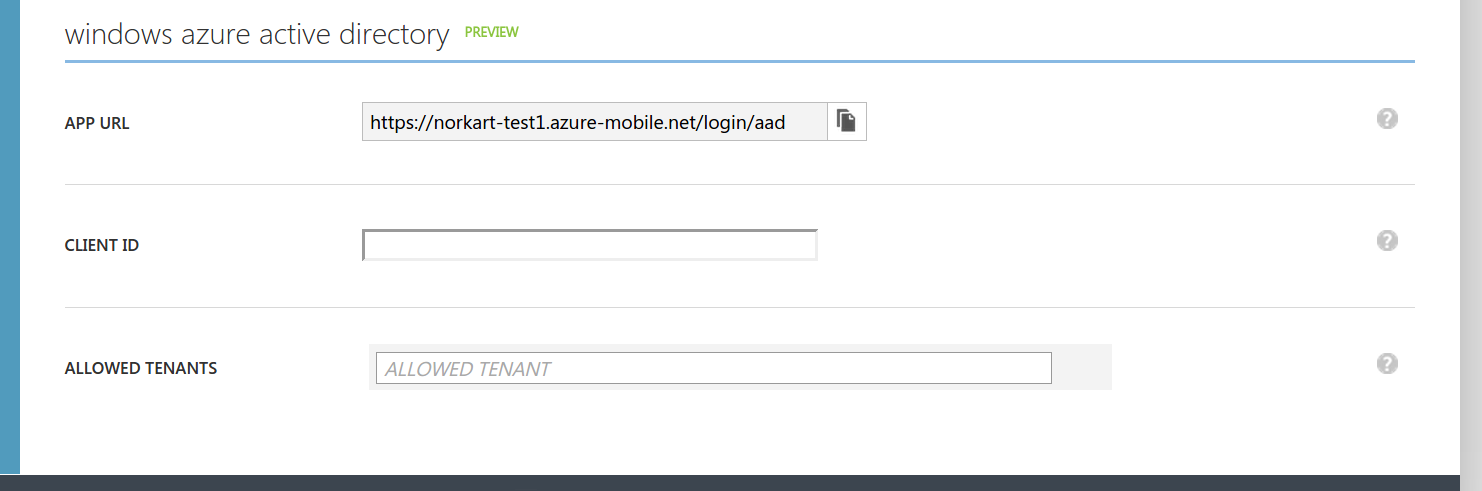
\includegraphics[scale=0.30]{graphics/veliedninger_implementeringAndroid/02-MobileServicesIdentity.png}}
    \caption{Kopier APP URL'en}
    %\label{fig:MobileServices}
\end{figure}
\\
\item Gå inn i den Azure Active Directory du ønsker skal ha tilgang og velg applications.
\\
\begin{itemize}
\item Klikk “ADD” nederst for og legge til en ny applikasjon.
\item Velg “Add an application my organization is developing”
\item Angi navnet applikasjonen skal ha i din Azure Active Directory
\item Velg “WEB APPLICATION AND/OR WEB API”
\item Klikk neste og angi den kopierte APP URL’n i begge boksene. 
\end{itemize}
\bigskip



\item Nå er applikasjonen lagt til i din Azure Active Directory, du skal nå hente ut “Client ID” for applikasjonen, for og knytte applikasjonen i Azure Active Directory sammen med Azure Mobile Services. 
\\
\begin{itemize}
\item Klikk på configure og scroll ned til “CLIENT ID”, kopier denne.
\item Gå tilbake til Azure Mobile Services, finn appen du kopierte URL’en fra tidligere, velg identity og scroll ned windows azure active directory, lim inn “CLIENT ID” i boksen under APP URL. 
\end{itemize}
\bigskip
\begin{figure}[H]
    \centering
    \setlength{\fboxsep}{0pt}%
    \setlength{\fboxrule}{1pt}%
    \fbox{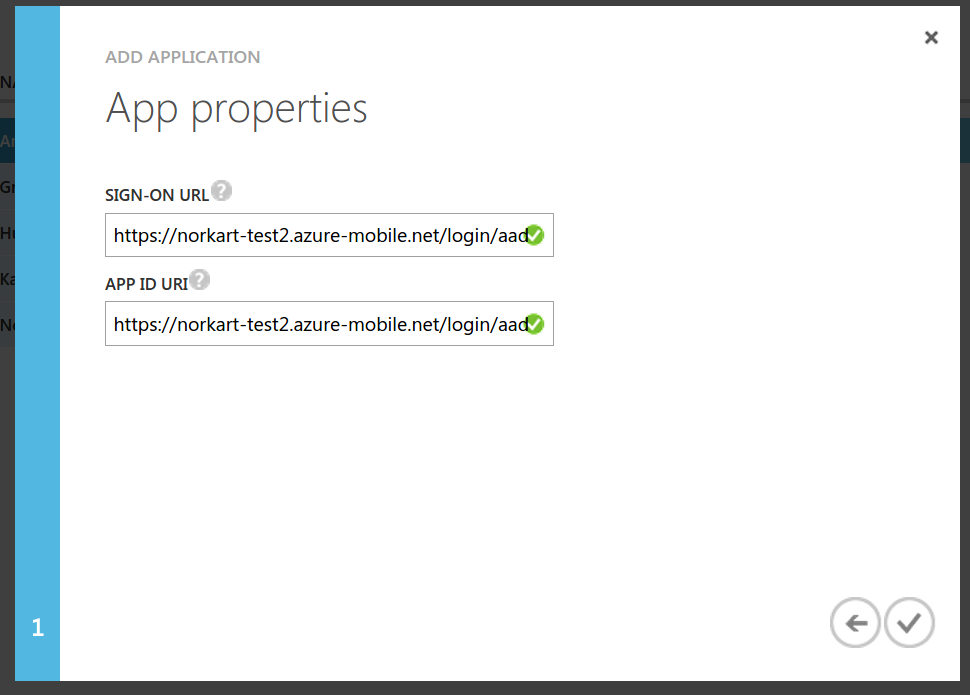
\includegraphics[scale=0.30]{graphics/veliedninger_implementeringAndroid/02-App-properties.png}}
    \caption{Fyll inn URL i begge feltene}
    %\label{fig:MobileServices}
\end{figure}
\\
\item For at du skal kunne logge inn med domenet angitt i din Azure Active Directory må du hente ut dette domenet fra Azure Active Directory og lime det inn i Azure Mobile Services. 
\\
\begin{itemize}
\item Gå til din Azure Active Directory, klikk på “DOMAINS”. 
\item Om du ikke har opprette egne domener vil det være angitt et standard domene. Kopier de domenene du ønsker skal ha tilgang til appen. (kan fortsatt ikke logge inn uten godkjent bruker).
\item Gå til Azure Mobile Services, velg applikasjonen, velg Identity, scroll ned til Windows Azure Active Directory og lim inn domenene i “ALLOWED TENANTS”
\end{itemize}
\bigskip
\begin{figure}[H]
    \centering
    \setlength{\fboxsep}{0pt}%
    \setlength{\fboxrule}{1pt}%
    \fbox{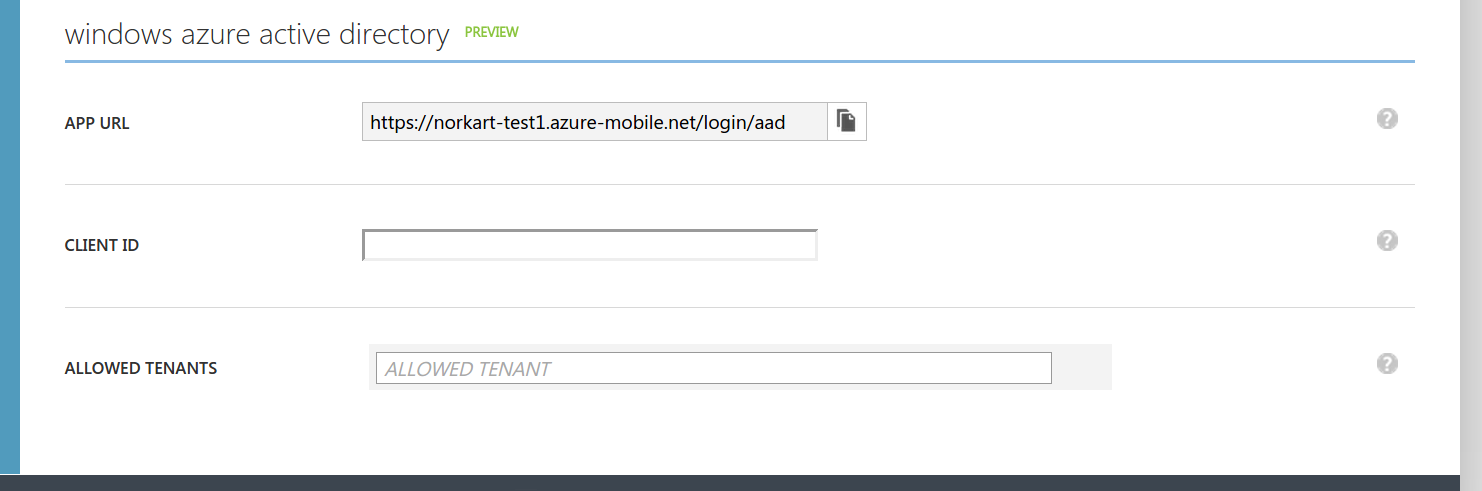
\includegraphics[scale=0.30]{graphics/veliedninger_implementeringAndroid/02-MobileServicesIdentity.png}}
    \caption{Fyll inn app ID og domener}
    %\label{fig:MobileServices}
\end{figure}

\\
\item Vi skal nå hindre andre brukere enn de som er autentiserte og endre data i databasen. 
\begin{itemize}
\item Gi i Azure Mobile Services, velg applikasjonen du skal endre, velg “DATA” derretter “PREMISSIONS” 
\item Endre alle rettighetene til “Only Authenticated Users”
\item Husk å klikke “SAVE” nederst etter at du har endret.
\end{itemize}
\bigskip
\begin{figure}[H]
    \centering
    \setlength{\fboxsep}{0pt}%
    \setlength{\fboxrule}{1pt}%
    \fbox{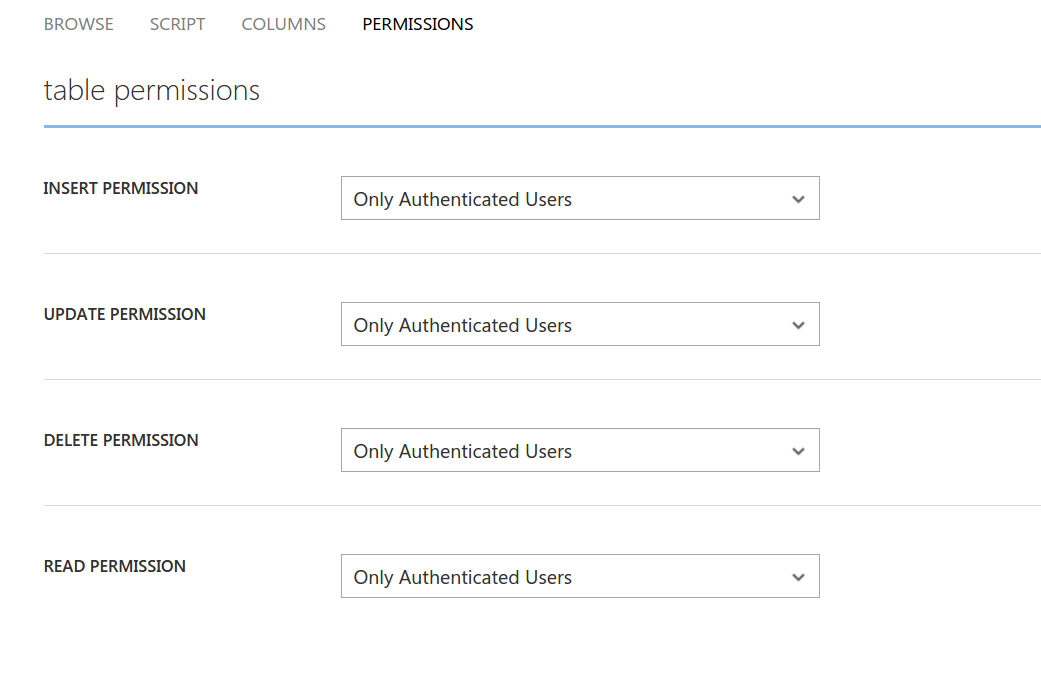
\includegraphics[scale=0.30]{graphics/veliedninger_implementeringAndroid/02-App-premissions.png}}
    \caption{Endre alle "table premissions"}
    %\label{fig:MobileServices}
\end{figure}

\\
\item Vi skal nå legge autentisering inn i app koden i Android studio. Endringene vi gjør her refererer til filnavnet i eksempelprosjektet. Om du ikke bruker eksempelprosjektet legg dette inn i klassen hvor “public void onCreate()” ligger. 
Legg til følgende biblioteker for import.
\\
\begin{lstlisting}[numbers=left, captionpos=b,   caption={Eksempel som viser hvilke biblioteker som bør importeres.}, ]
    
import java.util.concurrent.ExecutionException;
import java.util.concurrent.atomic.AtomicBoolean;

import android.content.Context;
import android.content.SharedPreferences;
import android.content.SharedPreferences.Editor;

import com.microsoft.windowsazure.mobileservices.authentication.MobileServiceAuthenticationProvider;
import com.microsoft.windowsazure.mobileservices.authentication.MobileServiceUser;
\end{lstlisting}
\\
\item Derretter legg til “authenticate()” klassen i samme filen. Kopier inn eksempelkoden nedenfor. Legg merke til at denne koden kan avvike fra veiledninger på nettet, ettersom det her er spesifisert WindowsAzureActiveDirectory som identity provider. 
\\
\begin{lstlisting}[numbers=left, captionpos=b,   caption={Eksempel som viser hvordan authenticate klassen kan se ut.}, ]

private void authenticate() {
    // Login using the Azure AD provider

    ListenableFuture<MobileServiceUser> mLogin = 
    mClient.login(
        mobileServiceAuthenticationProvider.WindowsAzureActiveDirectory);
    
    Futures.addCallback(mLogin, 
        new FutureCallback<MobileServiceUser>() {
        
        @Override
        public void onFailure(Throwable exc) {         
            createAndShowDialog((Exception) exc, "Error");
        }           
        
        @Override
        public void onSuccess(MobileServiceUser user) {
            createAndShowDialog(String.format(
                "You are now logged in - %1$2s",
                user.getUserId()), "Success");
            createTable();  
        }
    });     
}

\end{lstlisting}
\\
\item Derretter skal vi legge til authenticate() klassen. Om du bruker et annet prosjekt enn eksempelprosjektet vil det trolig og legge dette inn etter at du har initert alle objekter men ikke begynt og kjøre noe logikk operasjoner. For demoprosjektet legger vi det inn rett etter at vi har initiert MobileServiceClient i onCreate(); klassen, derretter flytter vi de kodelinjene som lå under MobileServiceClient initieringen ned i en egen klasse som vi kaller createTable(); 
\\
\begin{lstlisting}[numbers=left, captionpos=b,   caption={Eksempel som viser hvordan onCreate() klassen ser ut etter at kode er flytte til en egen createTable() klasse.}, ]

try {
   // Create the Mobile Service Client instance, using the provided
   
   // Mobile Service URL and key
   mClient = new MobileServiceClient(
        "https://norkart-test1.azure-mobile.net/",
        "nSxoADeTLiHClFQShuomNyfOeSGAQL23",
        this).withFilter(new ProgressFilter());
   
   authenticate();
   
   } catch (MalformedURLException e) {
        createAndShowDialog(new Exception("There was an error creating 
        the Mobile Service. Verify the URL"), "Error");
}
\end{lstlisting}
\\
\begin{lstlisting}[numbers=left, captionpos=b,   caption={Eksempel som viser hvordan createTable() klassen kan se ut.}, ]

private void createTable() {

    // Get the Mobile Service Table instance to use
    mToDoTable = mClient.getTable(ToDoItem.class);

    mTextNewToDo = (EditText) findViewById(R.id.textNewToDo);

    // Create an adapter to bind the items with the view
    mAdapter = new ToDoItemAdapter(this, R.layout.row_list_to_do);
    ListView listViewToDo = (ListView) findViewById(R.id.listViewToDo);
    listViewToDo.setAdapter(mAdapter);

    // Load the items from the Mobile Service
    refreshItemsFromTable();
}
\end{lstlisting}
\\
\item Nå skal du kunne kjøre appen og måtte oppgi identity provider for og få logget inn. \\
\item Det er fortsatt mulig å lure seg unna autentiseringen, da vil applikasjonen krasje når den ikke får svaret den forventer fra databasen. Du kan enten legge inn en egen sjekk som sjekker om du er autentisert eller ikke. Alaternativt kan du be applikasjonen avslutte seg selv om brukeren skulle forsøke å omgå autentiseringen. Dette kan du gjøre ved å legge til en finish(); i callBack exception i authenticate() klassen slik som angitt nedenfor.
\\
\begin{lstlisting}[numbers=left, captionpos=b,   caption={Eksempel som viser hvordan onFailure() kan se ut om det legges til en finish(); .},]

Futures.addCallback(mLogin, new FutureCallback<MobileServiceUser>() {
  @Override
  public void onFailure(Throwable exc) {
      createAndShowDialog((Exception) exc, "Error");
      finish();
  }

  @Override
  public void onSuccess(MobileServiceUser user) {
      createAndShowDialog(String.format(
          "You are now logged in - %1$2s",
          user.getUserId()), "Success");
      createTable();
  }
});

\end{lstlisting}
\\
\item Nå skal du kunne logge inn i applikasjonen. Det er ikke enda lagt til noen logg-ut knapp. For å teste at du kan logge inn med ulike brukere må du fjerne appdata i innstillinger for applikasjonen i android systemet. 
\end{enumerate}
